\chapter{Methodology}

\section{Overview of Similar Experiment}

Although this work has a slightly different aim than \cite{Abramova2014}'s stated purpose, this paper aims to follow \cite{Abramova2014}'s methodology closely enough as to anchor its results to a cross-section of similar work that has been done.  This work assumes that an in-situ storage application in the realm of \gls{iot} implies a small database, in this case represented by 1 million records, as opposed to 10 million or 100 million or more.  Although Abramova’s paper seems to imply there is feasibility for large database with many, many nodes given the right balance, this work focuses more on the initial impact to performance of introducing less-capable hardware in order to lighten costs or actual physical weight for an application that would see this as a benefit.

Using standard workloads A, C, and E from the popular \gls{ycsb}, the authors of \cite{Abramova2014} examined and evaluated Cassandra’s scalability over “database [sizes] and cluster sizes” \cite{Abramova2014}.  The authors found that this trend, depicted in Figures \ref{fig:wla_fig1}, \ref{fig:wlc_fig1}, and \ref{fig:wle_fig1} did not necessarily hold true across database sizes, that in fact for larger database sizes of 10 million and 100 million records, 3 node clusters performed better than both a single node cluster and a 6-node cluster.  The authors concluded that for sufficiently small databases, which is the likely case for \gls{iot}, more nodes imply more time to execute, which overwhelms any advantageous parallelism that may ensue with increasing nodes.

Because there are so many variables that can be at work, this work aims to anchor its results by replicating part of Abramova’s study.  The extent of the details of the network in \cite{Abramova2014} is detailed below:  

"The characteristics of nodes used are, as follows: Node 1 – Dual Core (3.4 GHz), 2GB RAM and disk with 7200 rpm; Node 2 – Dual Core (3.4 GHz), 2GB RAM and disk with 7200 rpm; Node 3 – Dual Core (3.4 GHz), 2GB RAM and disk with 7200 rpm; Node 4 – Dual Core (3.0 GHz), 2GB RAM and disk with 7200 rpm; Node 5 – Dual Core (3.0 GHz), 2GB RAM and disk with 7200 rpm; Node 6 – Virtual Machine with one Core (3.4 GHz), 2GB RAM and disk with 7200 rpm." \cite{Abramova2014}

The results of Workloads A, C, and E in \cite{Abramova2014} are depicted in Figures \ref{fig:wla_fig1}, \ref{fig:wlc_fig1}, and \ref{fig:wle_fig1} respectively, all depicting a positive correlation between execution time and the number of nodes.  The actual values are depicted in \ref{table:previous_paper_results}

\begin{table}
\begin{center}
 \begin{tabular}{||c c c||} 
 \hline
Nodes & Workload & [OVERALL] RunTime(ms) \\ [0.5ex] 
 \hline\hline
1 & a & 58430\\ 
 \hline
3 & a & 65650\\ 
 \hline
6 & a & 87310\\ 
 \hline
1 & c & 88000\\ 
 \hline
3 & c & 90210\\ 
 \hline
6 & c & 118090\\ 
 \hline
1 & e & 223180\\ 
 \hline
3 & e & 330820\\ 
 \hline
6 & e & 404660\\ 
 \hline
\end{tabular}
\end{center}

\caption{Results from \cite{Abramova2014} for 1 million record size database}
\label{table:previous_paper_results}
\end{table}

\begin{figure}[h]
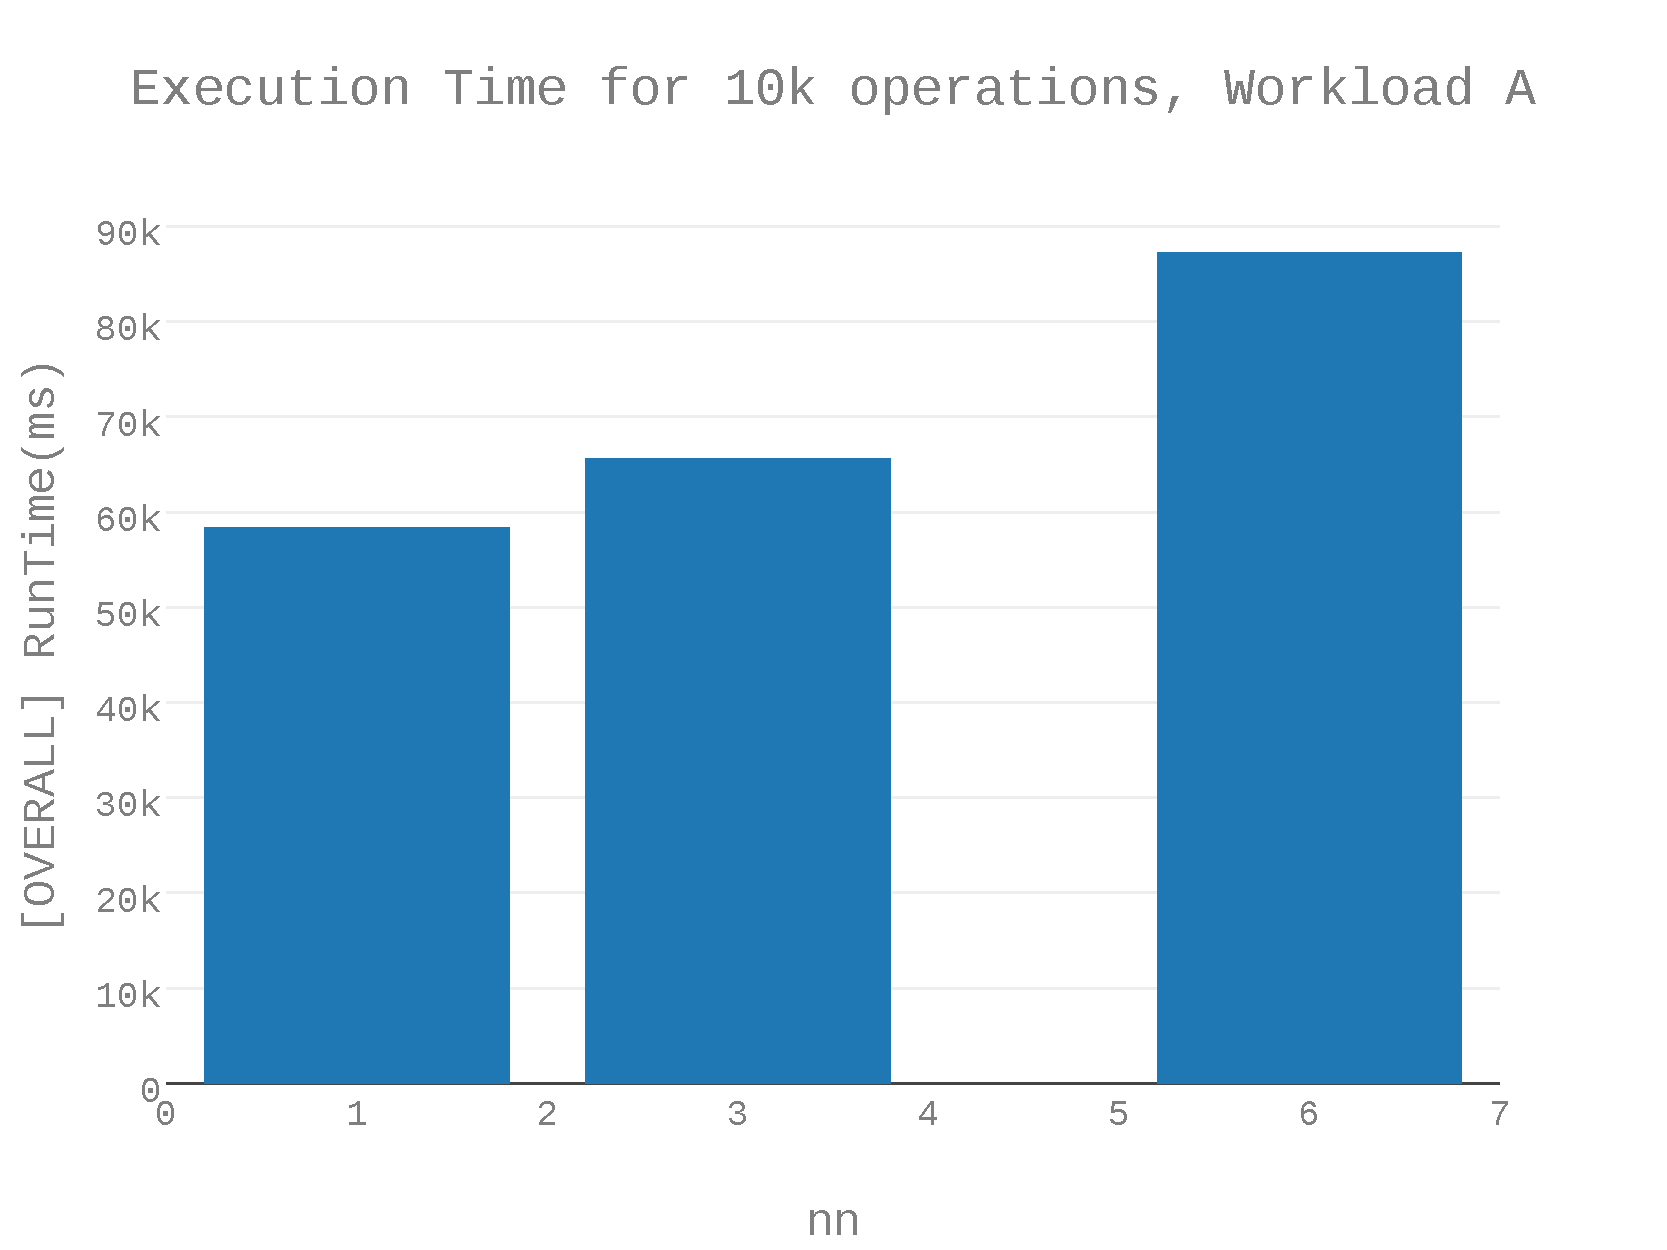
\includegraphics[width=3.5in]{Figures/figures-wla_fig1.pdf}

\caption{Cross Section of Results Imported from \cite{Abramova2014}.  This figure shows the execution time reported for 10,000 operations of Workload A over three given configurations: a network with only one (1) node, a network with 3 nodes, and a network with 6 nodes.}

\label{fig:wla_fig1}
\end{figure}

\begin{figure}[h]
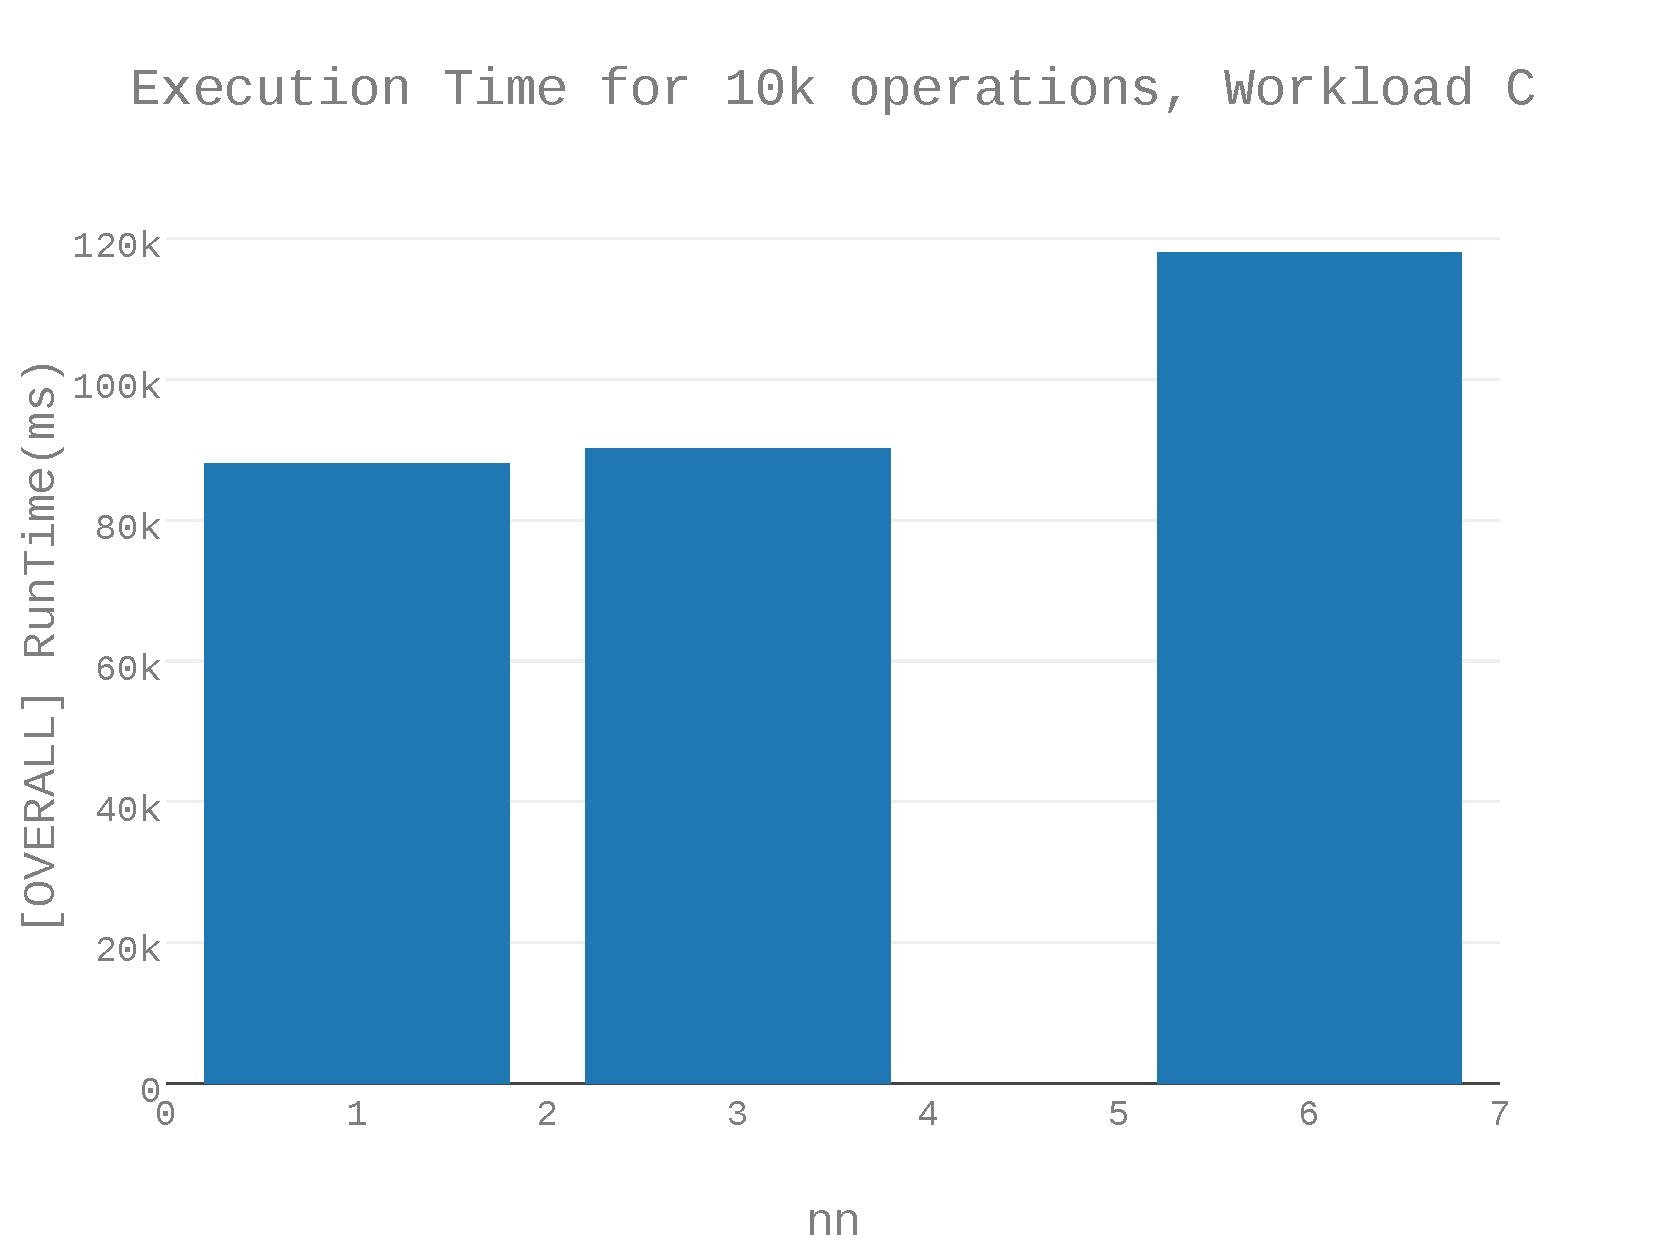
\includegraphics[width=3.5in]{Figures/figures-wlc_fig1.pdf}

\caption{Cross Section of Results Imported from \cite{Abramova2014}.  This figure shows the execution time reported for 10,000 operations of Workload C over three given configurations: a network with only one (1) node, a network with 3 nodes, and a network with 6 nodes.}

\label{fig:wlc_fig1}
\end{figure}

\begin{figure}[h]
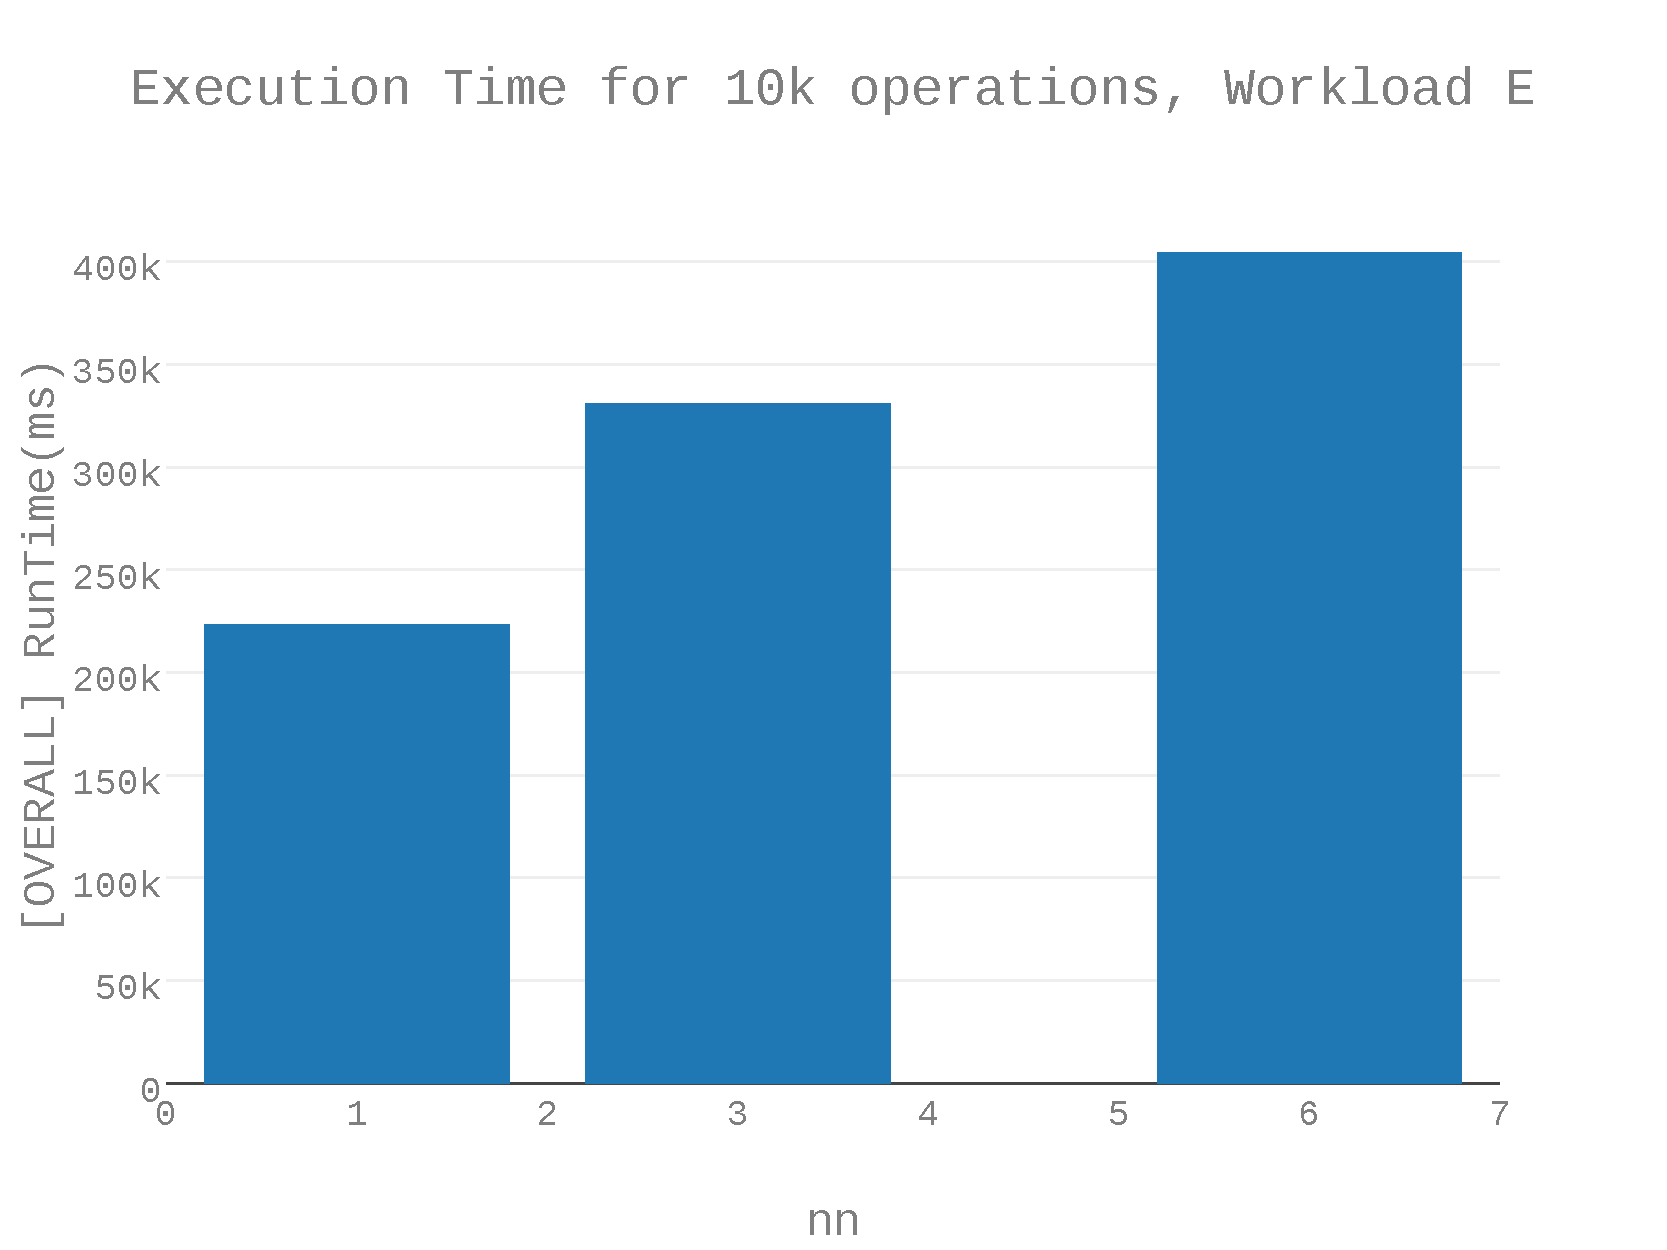
\includegraphics[width=3.5in]{Figures/figures-wle_fig1.pdf}

\caption{Cross Section of Results Imported from \cite{Abramova2014}.  This figure shows the execution time reported for 10,000 operations of Workload E over three given configurations: a network with only one (1) node, a network with 3 nodes, and a network with 6 nodes.}

\label{fig:wle_fig1}
\end{figure}

\section{Objective of This Set of Experiments}

The objective of this experiment is to characterize varying configurations for Cassandra.  This characterization will be in service of assessing the utility of Cassandra on the Raspberry Pi 2, which will in turn be an indicator toward the greater population of both distributed databases, archetype Cassandra, and hardware of archetype Raspberry Pi.

We aim to recreate results in \cite{Abramova2014} and then extend these experiments for a better characterization for \gls{iot}. In doing so, we answer the following research questions:
\begin{itemize}
\item Research Question 1: How much is the execution time for a given number of operations extended in the system under test using workload A (reads/updates)? 
\item Research Question 2: How much is the execution time for a given number of operations extended in the system under test using workload C (reads)?
\item Research Question 3: How much is the execution time for a given number of operations extended in the system under test using workload E (insert/scans)?
\item Research Question 4: And finally, how much is the execution time for a given number of operations extended in the system under test using custom workload I, the anticipated representative of in-situ distributed database \gls{iot} application?
\end{itemize}

To answer each of these questions, we aim for the following:
\begin{itemize}
\item Following the methodology, modified from \cite{Abramova2014}, observe and analyze the results of running the \gls{ycsb} for (at least) 1, 3 and 6 node networks for 2GB and a database size of 1 million records.
\item Extend the 2GB \gls{ram} virtual node: Vary the virtual machine's allotted \gls{ram} for similar \gls{iot} sizes of memory (512MB, 1GB, 4GB).  Observe and analyze for any effect.
\item Extend to Raspberry Pi 2 modules, which have 1GB of memory.  Observe any differences.
\item Extend to a wireless \gls{lan}.  Observe any differences.
\end{itemize}

\section{Expectations}

The results of these experiments are anticipated to be within reasonable bounds of previous work \cite{Abramova2014}.  The results are not, however, expected to provide enough data points to provide a utilitarian mathematical model.  Such a model is alluded to in future work.

\section{System Boundaries}

Virtual machine nodes were contained in a single laptop.  The wired \gls{lan} experiments were performed with all nodes and the associated router within about 3 meters of one another on a dedicated \gls{lan}.  Likewise, the wireless \gls{lan} experiments were performed with all nodes and the router within a radius of 3 meters on a dedicated and secured \gls{lan}.  The experiments were done in a residential, suburban area. The network was periodically monitored for unexpected hosts.  

\section{Experimental Limitations, Nuisance Factors, Known/Suspected Interactions}

The amount of interference on the \gls{ism} band could not be controlled.  It is left to the assumptions that any variation in interference was negligible between any two trials.

The laptop running the \gls{ycsb} may have been running other minor programs or other processes to a limited extent.  No experiments were done to determine if this would have a significant effect, and this was not strictly controlled.

\section{Coordination}

\subsection{Ethernet \gls{lan}}

No coordination was needed.  This network was physically isolated and no additional traffic was expected to interfere with it.

\subsection{Wireless \gls{lan}}

Because the scale and timing of this experiment was limited, there was no formal coordination needed.  However, because a larger experiment could possibly fill up one (or more) frequency channels, one must be courteous of the environment.  An extended test would not be appropriate in an uncontrolled environment.

\section{Treatments, Independent Variables}

The independent variables of interest are the node type and link type.  Node type is characterized by memory, or \gls{ram}, processor speed, and \gls{io} rates, and are represented by virtual nodes and the Raspberry Pi.

The link types are the internal nodes on the virtual machine network, Ethernet links, and wireless 802.11 links.

There are many other factors at work, but other factors, like workload, are only varied to give appropriate context to the variance in node type and link type. 

\section{Factors}

\subsection{Hard Disk Storage: \gls{sd} Card}

The manufacturer and model for each \gls{sd} card was kept constant for each node.  The details can be found in \ref{table:sd_card_specs}

\begin{table}
\begin{center}
 \begin{tabular}{||c c||} 
 \hline
 Specification & Value \\ [0.5ex] 
 \hline\hline
 Capacity & 16 GB \\ 
 \hline
 Read Speed & up to 90 MB/s \\
 \hline
 Write Speed & up to 40 MB/s \\ 
 \hline
 Video Speed & C10 U3 \\ [1ex] 
 \hline
\end{tabular}
\end{center}

\caption{Specifications for SD Cards \cite{SanDiskCard}}
\label{table:sd_card_specs}
\end{table}


\subsection{Database Size}

This work assumes that an in-situ storage application in the realm of \gls{iot} implies a small database, in this case represented by 1 million records, as opposed to 10 million or 100 million or more.  Although Abramova’s paper seems to imply there is feasibility for large database with many, many nodes given the right balance, this work focuses more on the initial impact to performance of introducing less-capable hardware in order to lighten costs or actual physical weight for an application that would see this as a benefit.

\subsection{Number of Operations Per Trial}

The results in \cite{Abramova2014} report an execution time after 10,000 operations, and the decision was made to keep this constant rather than vary the representative number of operations.  No explicit justification is given in \cite{Abramova2014} for the number 10,000, but it can be inferred that it lies somewhere between being too small to represent the population (1 or 2 operations would be too small), and a sample size too large, that which merited exchange with a smaller sample size that could achieve the same aim.  But, one can take a minor step further.

As a brief experiment, one can take a look at what it might look like to vary the sample size in a given trial, and how the execution time would vary over the sequence of trials.  The graph above shows this for two different configurations: 1GB and 4GB RAM on a virtual machine.  As expected, the execution time does reflect initial cache warm-up time, but then, more or less, reflects some sort of steady state, albeit oscillating performance.
It was also not made explicit whether or not the 10,000 operations represented one of many trials of 10,000 or represented a single and only trial.  For the purposes of exploring the data, this author chose to run 30 trials of 10,000 operations each.

\begin{figure}[h]
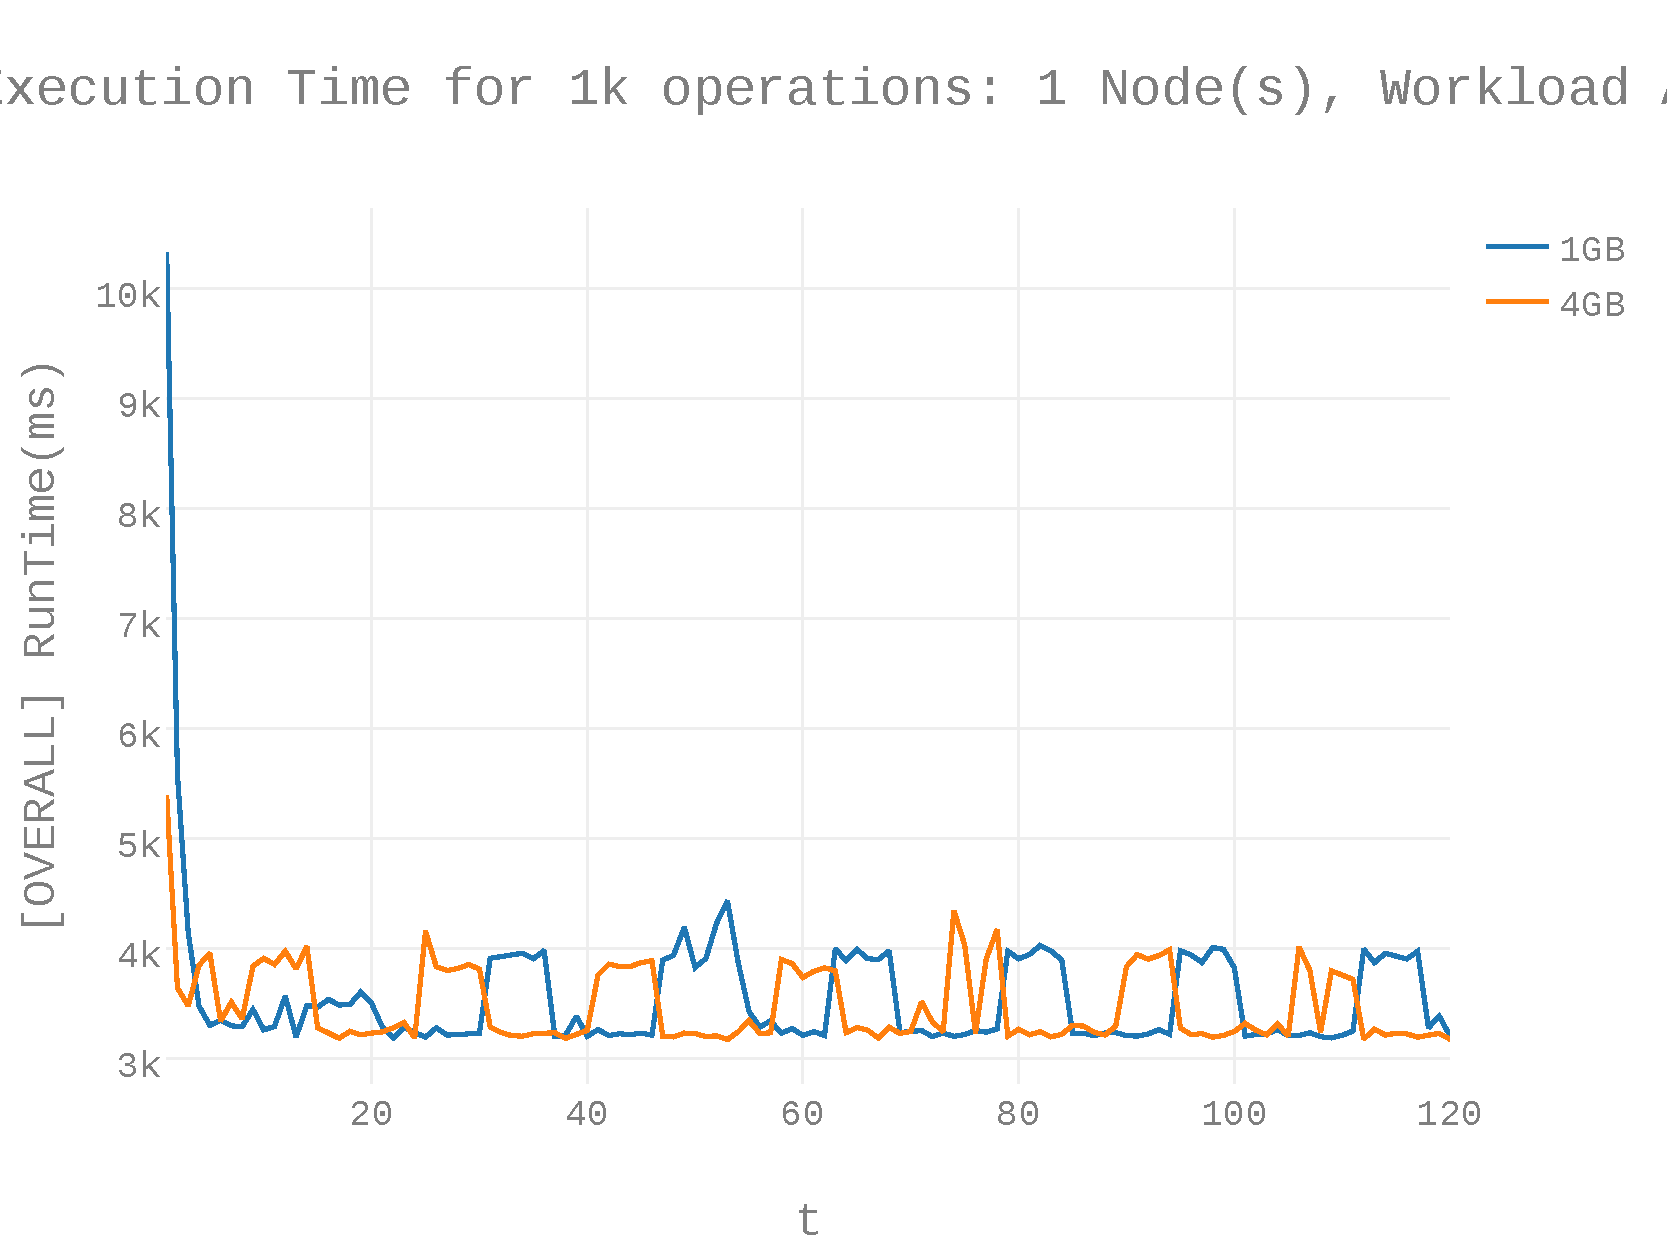
\includegraphics[width=3.5in]{Figures/figures-wla_fig2.pdf}

\caption{Two sample runs, adjusting the trials such that only 1000 operations of Workload A to a given trial.}

\label{fig:fig02}
\end{figure}

The oscillating behavior seen in trials 5 through 120 is distracting and risks inaccurate comparisons among configurations.  Although it is beyond the scope of this paper to determine the exact cause of this oscillation, one might consider that activities required for the operation of the database, such as compaction, the gossip protocol, and other operations compete with the reads and will contribute to continuous variation over time, and may affect performance measurements.  The reason for choosing 10,000 operations is not explicitly reported in \cite{Abramova2014}, but one may infer the reason is to integrate this variation to make better comparisons among configurations.  

\begin{figure}[h]
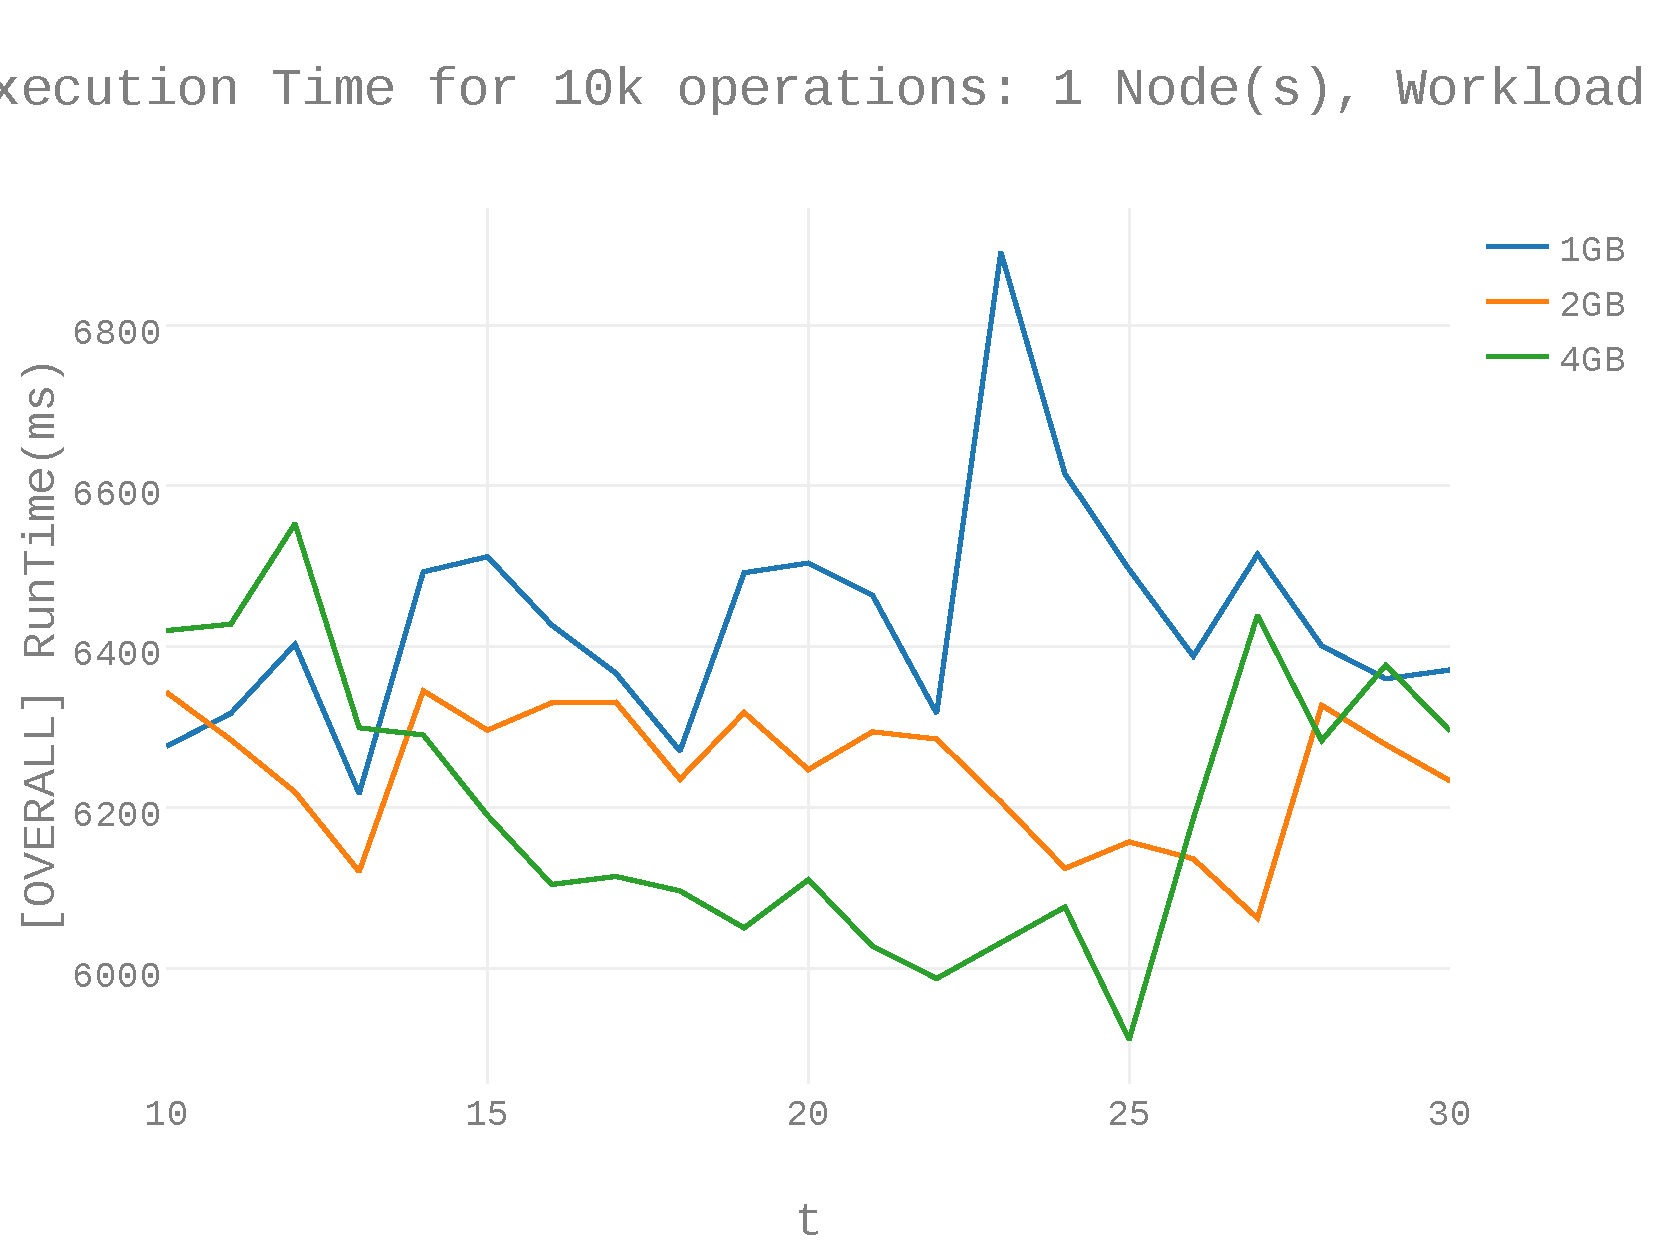
\includegraphics[width=3.5in]{Figures/figures-wla_fig3.pdf}

\caption{A series of trials for 1GB, 2GB, and 4GB \gls{ram} virtual machines.  The inset demonstrates that any pattern that could significantly distinguish one trial from another, such as the oscillation seen in \ref{fig:fig02} is integrated such that, after the cache warm-up period, the relative position of the trial does not predict the relative outcome.}

\label{fig:fig03}
\end{figure}

Contrast the 1k operation trials with the 10k operation trials depicted in \ref{fig:fig03}.  Here, at least with the naked eye, there is no oscillation, and most certainly not to the extent seen in the 1k trial case.  Whatever effected the oscillating behavior in the previous graph is integrated into the 10k trial case and is no longer a distraction to steady-state analysis, as each 10k operation trial soaks up, or rather integrates, the performance of quantity 10 1k operation trials.  Of course, more operations take longer to run, and thus the cost in testing time starts to curtail the value of integrating more trials.

\subsection{Workloads}

Just as in \cite{Abramova2014}, standard workloads A, C, and E were put to the test, while B, D, and F are saved for future work.  In addition, this paper introduces a custom workload, denoted I, to represent an \gls{iot} application, many inserts and few reads, a 99 percent to 1 percent ratio.

Standard workloads A, C, and E, from the \gls{ycsb} are summarized in Table \ref{table:std_workloads}.
\begin{table}
\begin{center}
 \begin{tabular}{||c c c c||} 
 \hline
 Workload & Read & Update & Scan \\ [0.5ex] 
 \hline\hline
 A & 0.5 & 0.5 & 0.0 \\ 
 \hline
 C & 1.0 & 0.0 & 0.0 \\
 \hline
 E & 0.0 & 0.0 & 1.0 \\ [1ex] 
 \hline
\end{tabular}
\end{center}

\caption{Standard \gls{ycsb} workloads used in this methodology.  Workload A consists of 50 percent reads and 50 percent updates.  Workload C consists of 100 percent reads.  Workload E consists of 100 percent scans.}
\label{table:std_workloads}
\end{table}

\begin{table}
\begin{center}
 \begin{tabular}{||c c c c c||} 
 \hline
 Workload & Read & Update & Scan & Insert \\ [0.5ex] 
 \hline\hline
 A & 0.50 & 0.50 & 0.00 & 0.00 \\ 
 \hline
 C & 1.00 & 0.00 & 0.00 & 0.00 \\
 \hline
 E & 0.00 & 0.00 & 1.00 & 0.00\\ 
 \hline
 I & 0.01 & 0.00 & 0.00 & 0.99 \\ [1ex] 
 \hline
\end{tabular}
\end{center}

\caption{Standard \gls{ycsb} workloads used in this methodology.  Workload A consists of 50 percent reads and 50 percent updates.  Workload C consists of 100 percent reads.  Workload E consists of 100 percent scans.  In addition, a custom workload I is summarized, which consists of 99 percent writes and 1 percent reads to represent \gls{iot}.}
\label{table:std_workloads_with_i}
\end{table}

In this experiment, we measure the total run time of a fixed number of operations of Workload A for various memory sizes. The choice of memory size is due to the expectations of \gls{iot} devices. The Raspberry Pi 2 and 3 have 1GB of memory and is our representative technology for \gls{iot}. The 4GB configuration can be considered be more representative of a low-end desktop, laptops, or virtual machine. The 2GB configuration is an intermediate stage that show an intermediate performance level and naturally, may represent the aim of future of \gls{iot} nodes. In addition, \cite{Abramova2014} used 2GB machines, which may help this work to be compared against existing work.

For this work, virtual nodes were created to match these characteristics to a reasonable extent.  Facing minimal propagation delay due to being connected on a nodal network, experiments with the virtual machines seek to place an upper limit on potential \gls{iot} performance expectations. Replicating the exact network in \cite{Abramova2014} is not absolutely necessarily, notwithstanding the details and materials available to do so are unavailable.

\subsection{Configuration of Cassandra}

Unless otherwise specified, the configuration of Cassandra, the keyspace, and the table within the keyspace are all held constant to their default values.  All three of these things can be configured hierarchically, and their configuration can affect the performance of Cassandra on a given load.  A skillful adjustment of these parameters can result in an optimized performance of Cassandra.

This paper aims to highlight the differences in varying hardware, and thus the exact configuration, despite that it might raise the absolute level of performance, is not expected to elevate the relative level of performance one would see shifting between, say a virtual node on a laptop and a Raspberry Pi module.

There are a few settings that had to be taken into account.  Denoted $commitlog\_total\_space\_in\_mb$, this will accumulate to an undesired level.  This was set to 512 MB in the Cassandra configuration file, cassandra.yaml.  (Changing this to 256 MB for the 512 \gls{ram} case did not correct the error mentioned above.)  Also, to prevent the accumulation of space, the setting $auto\_snapshot$ to false in configuration file cassandra.yaml.  Having $auto\_snapshot$ set to true automatically backs up, or saves a snapshot of, the data on Cassandra.  For a limited-capacity node, this is a luxury one cannot afford.

The configuration files can be found among the appendices.

\subsection{Threads in the \gls{ycsb}}

The number of threads was kept constant at 1, although by increasing the number of threads one could achieve greater throughput.  However, since it was desired to compare different calculations, the default was retained for all configurations.

It may be worth noting that for loads, this number was increased for practical reasons.  However, pure writes were not measured in these experiments, only the defined workloads A, C, E, and custom workload I.

\section{Assumptions}
\label{Assumptions}

Naturally, in order to perform the experiment and evaluate the results, some assumptions had to be made.
Investigation into any of these assumptions may be a lead into future work.

\begin{enumerate}

\item The benchmark represents the application, which assumes a simple schema.  In other words, Cassandra's performance is not particularly sensitive to the schema.

\item There is no active attacker or intrusion into the local area networks.  Both the local area networks are isolated.

\item There are no errors with the custom benchmark that would skew the results.  Any error is due to the fact that the system's limits have been reached.

\item There are no bugs in the benchmark that would skew the results.

\item Effects on the network due to distance are negligible.

\item This experiment assumes that nodes are homogeneous.  The basis for this assumption is that all nodes have been specified to the same model of Raspberry Pi 2.  The same make and model for the SD Cards have been used.  The image upon the SD Cards has been copied and only adjusted to account for specific, differentiated IP addresses.

\item This experiment assumes an uninterrupted power supply.  Power supply has no bearing on Cassandra’s performance on the hardware cluster, and is not measured nor accounted for in the model.

\item This experiment assumes an uninterrupted power supply.  Power is not measured nor accounted for in the model.  As long as the power has been turned on, it stays on, and fluctuations in voltage or any kind of imperfections in the power supply are negligible with respect to Cassandra's performance.

\item Although the ISM band is unregulated, this experiment assumes invariant interference from other emitters.  The experiment assumes an urban to suburban environment.  In other words, congestion that overwhelms Cassandra's performance can be assumed to be rare with respect to the population, and is ignored for the purposes of the experiment.

\item Another note on interference for the wireless configurations.  This experiment assumes invariant interference regardless of how much data is being written to the table in Cassandra. For the given pet application, collecting WiFi signals, the benchmark may be related to the amount of expected interference.  Probe requests can be indicative of WiFi traffic with which Cassandra might be competing, but this would require further investigation.  

\end{enumerate}

\section{Experimental Setup}

The experiments performed can be summarized in Table \ref{table:topologies}.
\begin{table}
\begin{center}
 \begin{tabular}{||c c c||} 
 \hline
 Communication (nm) & Platform (nt) & Assigned RAM \\ [0.5ex] 
 \hline\hline
 Nodal & Virtual Machine & 1 GB \\ 
 \hline
 Nodal & Virtual Machine & 2 GB \\
 \hline
 Nodal & Virtual Machine & 4 GB \\
 \hline
 Ethernet LAN & Raspberry Pi & 1 GB \\
 \hline
 802.11 LAN & Raspberry Pi & 1 GB \\
 \hline
\end{tabular}
\end{center}
\caption{This table summarizes each network topology that was explored in each research question.  The \gls{ram} was varied on the Virtual Machines.  It was not of interest to attempt to vary the \gls{ram} on the Raspberry Pi nodes.}
\label{table:topologies}
\end{table}



\subsection{Virtual Node Setup}

For this work, virtual nodes were created to match these characteristics to a reasonable extent.  Facing minimal propagation delay due to being connected on a nodal network, experiments with the virtual machines seek to place an upper limit on potential \gls{iot} performance expectations. Replicating the exact network in \cite{Abramova2014} is not absolutely necessarily, notwithstanding the details and materials available to do so are unavailable.

On a 64-bit 31.1GiB RAM laptop with Intel Core i7-4910MQ 2.90GHz 8-core central processing unit, six (6) identical virtual machines were created in software VirtualBox.  Each machine consisted of Ubuntu 64 bit machine was was allocated 8 GB of hard drive disk space.  The full details for these machines, reported by means of the lshw Linux command, are located among the appendices.  Also in VirtualBox, a host-only network entitled vboxnet0 was instantiated, to which all six machines were connected.

The \gls{ycsb} was installed and run on the host laptop.  PyCharm drove a terminal process, which in turn drove the \gls{ycsb} software.

To further paint the picture of the network setup, the \gls{ip} addresses are included in Table \ref{table:ip_addresses_vm}

\subsection{Ethernet \gls{lan} Setup}

The wiring of the Ethernet \gls{lan} is depicted in Figure \ref{fig:topology_for_ethernet_setup}.  Note that for the Ethernet set up, the wireless capability for the home router was switched OFF.

All nodes, including the laptop used to execute the \gls{ycsb}, were on the same network.  Their \gls{ip} addresses are listed in Table \ref{table:ip_addresses_rp}.

\begin{table}
\begin{center}
 \begin{tabular}{||c c c c||} 
 \hline
 Node & Host Name & IP Address & Model \\ [0.5ex] 
 \hline\hline
 Node 1 & raspberrypi0 & 192.168.1.100 & 2B \\ 
 \hline
 Node 2 & raspberrypi1 & 192.168.1.101 & 2B  \\
 \hline
 Node 3 & raspberrypi2 & 192.168.1.102 & 2B \\
 \hline
 Node 4 & raspberrypi3 & 192.168.1.103 & 2B \\
 \hline
 Node 5 & raspberrypi4 & 192.168.1.104 & 2B \\
 \hline
 Node 6 & raspberrypi9 & 192.168.1.109 & 3 \\
 \hline 
 Laptop & daniel-ThinkPad-W541 &192.168.1.200 & - \\
 \hline
\end{tabular}
\end{center}
\caption{This table describes the \gls{ip} addresses in order to paint a further detailed understanding of network set up.  The netmask is 255.255.255.0}
\label{table:ip_addresses_rp}
\end{table}

\begin{table}
\begin{center}
 \begin{tabular}{||c c c||} 
 \hline
 Node & Host Name & IP Address \\ [0.5ex] 
 \hline\hline
 Node 1 & c0 & 192.168.56.100 \\ 
 \hline
 Node 2 & c1 & 192.168.56.101  \\
 \hline
 Node 3 & c2 & 192.168.56.102 \\
 \hline
 Node 4 & c3 & 192.168.56.103 \\
 \hline
 Node 5 & c4 & 192.168.56.104 \\
 \hline
 Node 6 & c5 & 192.168.56.105 \\
 \hline 
 Laptop & daniel-ThinkPad-W541 & 192.168.56.200 \\
 \hline
\end{tabular}
\end{center}
\caption{This table describes the \gls{ip} addresses in order to paint a further detailed understanding of network set up.  The netmask is 255.255.255.0}
\label{table:ip_addresses_vm}
\end{table}

\begin{figure}[h]
\centering
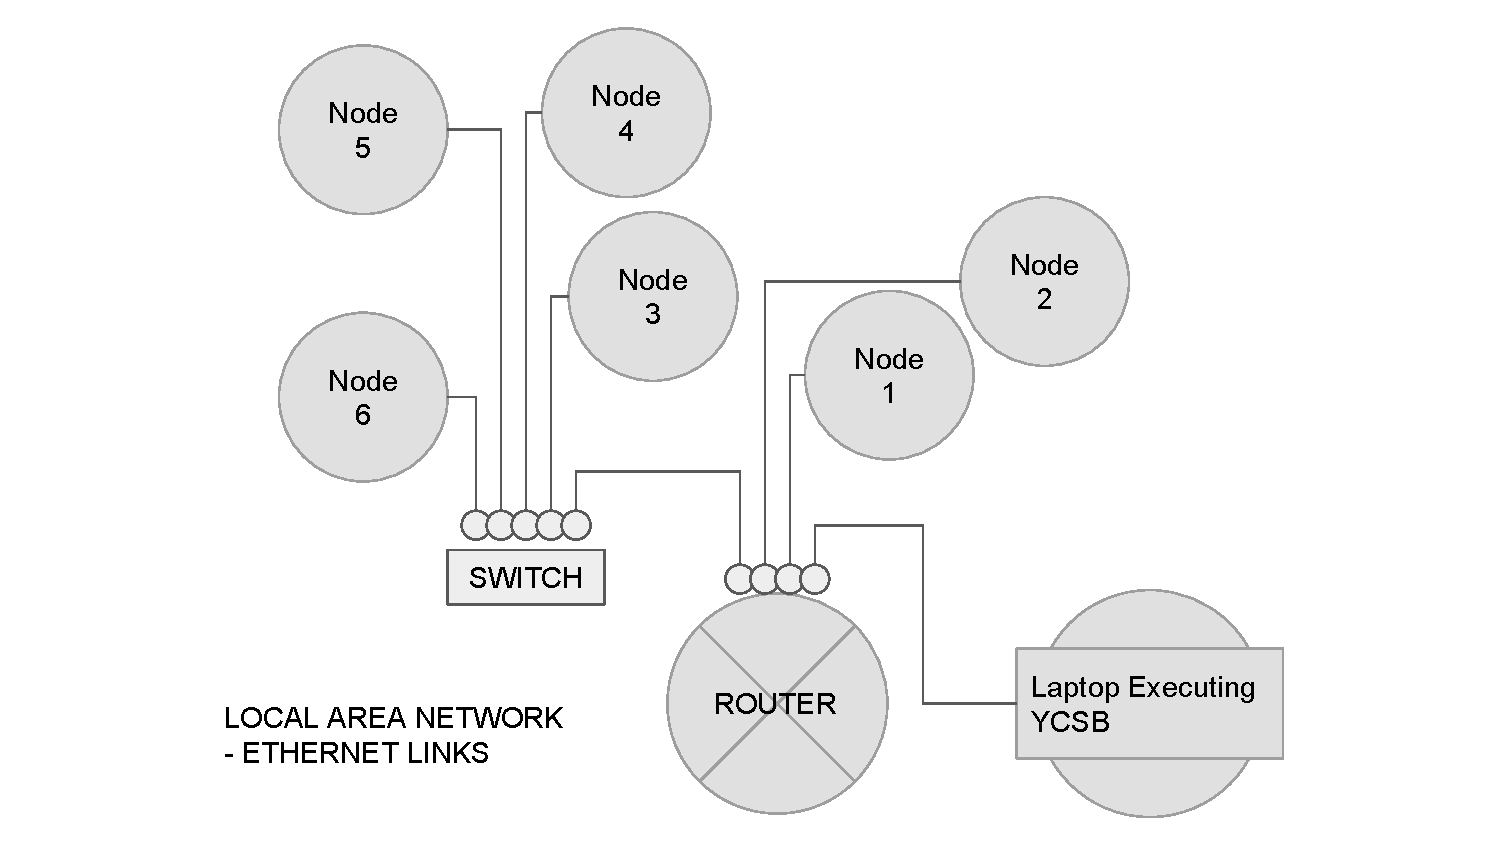
\includegraphics[width=7cm]{Figures/lan_eth.pdf}

\caption{Topology and Wiring for Ethernet Setup}

\label{fig:topology_for_ethernet_setup}
\end{figure}

\subsection{802.11 \gls{lan} Setup}

Table \ref{table:ip_addresses_rp_wireless} describes the local area network as the wireless the.  Note that for this setup, the Ethernet cables were physically unplugged.

To enable wireless links on the Raspberry Pi 2's, the Wi-Pi \gls{usb} module was utilized, with transmission speed capabilities listed at "11b – 1/2/5.5/11Mbps, 11g – 6/9/12/18/24/36/48/54Mbps, 11n – up to 150Mbps" \cite{RaspberryHut}.  The Raspberry Pi 3 model comes with its own built-in WiFi capabilities.

\begin{table}
\begin{center}
 \begin{tabular}{||c c c||} 
 \hline
 Node & Host Name & IP Address \\ [0.5ex] 
 \hline\hline
 Node 1 & raspberrypi0 & 192.168.1.130 \\ 
 \hline
 Node 2 & raspberrypi1 & 192.168.1.131  \\
 \hline
 Node 3 & raspberrypi2 & 192.168.1.132 \\
 \hline
 Node 4 & raspberrypi3 & 192.168.1.133 \\
 \hline
 Node 5 & raspberrypi4 & 192.168.1.134 \\
 \hline
 Node 6 & raspberrypi9 & 192.168.1.139 \\
 \hline 
 Laptop & daniel-ThinkPad-W541 &192.168.1.200 \\
 \hline
\end{tabular}
\end{center}
\caption{This table describes the \gls{ip} addresses in order to paint a further detailed understanding of network set up.  The netmask is 255.255.255.0}
\label{table:ip_addresses_rp_wireless}
\end{table}

\section{Execution}

The \gls{ycsb}, installed on the host laptop, is also run from the host laptop.  The \gls{ycsb} can be run from the terminal, but for convenience, a Python script was developed to drive a series terminal processes.

\section{Analysis}

For each experiment, the trials for each configuration will be reported as a summary of execution times for 10,000 operations.  All execution times will be reported in milliseconds.

\subsection{Response Variables}

The \gls{ycsb} reports a number of measured values, including operations per second and latency distribution (minimum, mean, 50 percentile or median, 75 percentile, 99 percentile, maximum).  The total execution time in milliseconds was chosen in order to keep the measured values true to the limits of the experiment.  Although operations per second and latency are more useful to know, since they are not confined to a fixed number of operations, the results in this paper are confined to 10,000 operations.  Although this paper aims to analyze results to reflect the steady state, this paper does not deny the possibility that variance in operations per second or variance in latency may result from variance in the number of operations (in this case, 10,000) per trial. 

\section{Cache Warm-Up Period and the Logic of Using the Median from This Point Forward}

Also, one can note in both Figure \ref{fig:fig02} and Figure \ref{fig:fig03}, that in the first five trials or so, one can observe the cache warm-up period.  This steep decline is expected due to the effect of the key cache, which is at it’s default setting: Cassandra sets the key cache to the either 5\% of the heap, or 100 MB, whichever is less.  In \cite{Abramova2014}, the key cache is reported to be at 100 MB.  The steady state operation is dependent on the keys requested, so for a workload like the YCSB, one would not expect a lot of variation.

Truncating the head of the trials, trials 1 though 9, the cache effect is no longer depicted, rendering an expectation of steady-state performance after cache warm-up.  This closer look indicates that varying \gls{ram} makes no significant difference in Cassandra’s performance.  This indicates that for the Raspberry Pi, and \gls{iot} devices in general, once a minimum threshold is reached in \gls{ram}, there are diminishing, if any, returns on performance for the potential inclusion of greater amounts of \gls{ram} on a piece of hardware. 

Taking the issues of oscillating behavior and cache warm-up period into account, we can remove them to find a stable viewing window into the behavior of the Cassandra database, as depicted in Figure \ref{fig:fig03}. Figure 4 shows the desired observation of the behavior in question for 1GB, 2GB ad 4GB memory sizes. We use this data to recreate Abramova’s work and extend it for other memory sizes.

Truncating the head of the trials, trials 1 though 9, the cache effect is no longer depicted, rendering an expectation of steady-state performance after cache warm-up.  This closer looks indicates that varying RAM makes no significant difference in Cassandra’s performance.  This indicates that for the Raspberry Pi, and IoT devices in general, once a minimum threshold is reached in RAM, there are diminishing, if any, returns on performance for the potential inclusion of greater amounts of RAM on a piece of hardware. 
This is the logic behind using the median to summarize the execution times.  The explanation here is the basis for the assumption that the median is a relevant summary statistic.  Of course, this is expected to hold true as long as there are at least 5 ‘steady-state’ data points to make up for the cache warm-up.

Another important observation here, is that once the cache effect is cropped out, there is no correlation between trials and the performance measurement.  This further supports that 10,000 operations, minus cache effect, does represent a steady state that is likely to extend beyond 10,000 operations.

This paper will then, for each workload, explore and compare the different network configurations, gauging the various conditional penalties that incur.  This paper will also gauge how Cassandra reacts having 1, 2, up through 6 nodes operating.  
